% article example for classicthesis.sty
\documentclass[10pt,a4paper]{article}
\usepackage{lipsum}
\usepackage{url}
\usepackage[nochapters]{classicthesis} % nochapters
% \usepackage[showframe=true]{geometry}  
\usepackage{changepage}
\usepackage{graphicx}
\usepackage{amsmath}


\begin{document}
\title{\rmfamily\normalfont\spacedallcaps{Homework for Neural Network Exam}} 
    \author{\spacedlowsmallcaps{Massimo Nocentini}} \date{\today}
    
    \maketitle

    %% \noindent\lipsum[1] Just a test.\footnote{This is a footnote.}      
    \begin{abstract}
      This article collects the work I did in order to support my
      Neural Network course final exam. The goal is to study neural networks
      using different training functions in order to test them against a dataset
      which holds datas about abalone. This short document describes our experience:
      we outline the problem and its application environment, the dataset used in
      experiments and a comparison of classification's results by different training functions.
      \end{abstract}
       
     

    \section{Problem description}
    
    We choose a classification problem in order to gain insights about neural networks.
    In particular, the dataset under study contains informations about abalone and
    the contained data comes from real measurements. The original article related to this
    dataset can be found in \cite{Nash-Sellers-Talbot-Cawthorn-Ford} and the dataset itself
    can be downloaded from \cite{ml-berkeley-dataset-url}. We report the original 
    problem description given in the article:
    \begin{quote}
    Predicting the age of abalone from physical measurements.  The age of
    abalone is determined by cutting the shell through the cone, staining it,
    and counting the number of rings through a microscope -- a boring and
    time-consuming task.  Other measurements, which are easier to obtain, are
    used to predict the age.  Further information, such as weather patterns
    and location (hence food availability) may be required to solve the problem.

    From the original data examples with missing values were removed (the
     majority having the predicted value missing), and the ranges of the
    continuous values have been scaled for use with an ANN (by dividing by 200).
    \end{quote}

    So, our goal is to classify abalone's age, in order to achieve this goal
    we tackle the dataset structure in the next section.

    \section{Dataset structure}

    The choosen dataset holds $4177$ samples and $8$ features variables and it 
    is structured according the following description:

    \begin{verbatim}
    Name            Data Type   Meas.   Description
    ----            ---------   -----   -----------
    Sex             nominal             M, F, and I (infant)
    Length          continuous  mm      Longest shell measurement
    Diameter        continuous  mm      perpendicular to length
    Height          continuous  mm      with meat in shell
    Whole weight    continuous  grams   whole abalone
    Shucked weight  continuous  grams   weight of meat
    Viscera weight  continuous  grams   gut weight (after bleeding)
    Shell weight    continuous  grams   after being dried
    Rings           integer             +1.5 gives the age in years
    \end{verbatim}

    With the following statistic summary:

    \begin{verbatim}
            Length  Diam    Height  Whole   Shucked Viscera Shell   Rings
    Min     0.075   0.055   0.000   0.002   0.001   0.001   0.002       1
    Max     0.815   0.650   1.130   2.826   1.488   0.760   1.005      29
    Mean    0.524   0.408   0.140   0.829   0.359   0.181   0.239   9.934
    SD      0.120   0.099   0.042   0.490   0.222   0.110   0.139   3.224
    Correl  0.557   0.575   0.557   0.540   0.421   0.504   0.628     1.0
    \end{verbatim}

    Response variable \emph{Rings} is the target of classification. 
    In our work we do not use each age value $v \in \lbrace 1, \ldots, 29 \rbrace$ 
    as classification bucket since having $29$ classes is quite dispersive.
    Thus we aggregate the available \emph{Rings} values in six classes, called \emph{One},
    \emph{Two}, \emph{Three}, \emph{Four}, \emph{Five} and \emph{Six} for simplicity, each of length five, 
    starting from zero, inclusive on the left. Formally, $\forall v \in Rings$ holds: 
    \begin{displaymath}
        \begin{split}
                v \in One &\leftrightarrow v \in \lbrace 0, \ldots, 4 \rbrace \\
                v \in Two &\leftrightarrow v \in \lbrace 5, \ldots, 9 \rbrace \\
                v \in Three &\leftrightarrow v \in \lbrace 10, \ldots, 14 \rbrace \\
                v \in Four &\leftrightarrow v \in \lbrace 15, \ldots, 19 \rbrace \\
                v \in Five &\leftrightarrow v \in \lbrace 20, \ldots, 24 \rbrace \\
                v \in Six &\leftrightarrow v \in \lbrace 25, \ldots, 29 \rbrace \\
        \end{split}
    \end{displaymath}

    \begin{table}
        \begin{tabular}{ c | c }
            Comprehensive distribution over $2924$ samples  &   Secret distribution over $1253$ samples \\
            \hline 
            \begin{tabular}{ l  r }
One & 39 (1.33 \%)\\
Two & 1463 (50.03 \%)\\
Three & 1240 (42.41 \%)\\
Four & 158 (5.40 \%)\\
Five & 21 (0.72 \%)\\
Six & 3 (0.10 \%)\\
\end{tabular} & \begin{tabular}{ l  r }
One & 26 (2.08 \%)\\
Two & 606 (48.36 \%)\\
Three & 521 (41.58 \%)\\
Four & 80 (6.38 \%)\\
Five & 18 (1.44 \%)\\
Six & 2 (0.16 \%)\\
\end{tabular} \\
            \hline
        \end{tabular}
      \caption{On the left: histogram of samples used for training after aggregation.
        On the right: histogram of samples kept secret after aggregation.}
      \label{fig:comprehensive-histograms}
    \end{table}

    In \autoref{fig:comprehensive-histograms} we report the distribution of samples against
    the six defined classes: we take apart the dataset in two partitions, the bigger one is
    used for training, on the other hand the smaller one contains samples kept secret
    in order to study how well a training function works when it sees a new sample not
    trained for.

    Dataset partitioning has been performed using the uniform distribution, and we 
    repeat partitioning until distributions shown in \autoref{fig:comprehensive-histograms}
    appeared, such that distribution of samples used for training is quite similar
    to distribution of samples kept secret.

    \begin{table}
      \begin{adjustwidth}{-4cm}{}
        \begin{tabular}{ l | l | l | l | l }
 & Backpropagation & RProp & SCG & LM \\
\hline
All & \begin{tabular}{ l  r }
One & 48 (1.15 \%)\\
Two & 2136 (51.14 \%)\\
Three & 1978 (47.35 \%)\\
Four & 15 (0.36 \%)\\
Five & 0 (0.00 \%)\\
Six & 0 (0.00 \%)\\
\end{tabular}
& \begin{tabular}{ l  r }
 One & 13 (87.8 \%)\\
 Two & 13 (87.8 \%)\\
 Three & 13 (87.8 \%)\\
 Four & 13 (87.8 \%)\\
 Five & 13 (87.8 \%)\\
 Six & 13 (87.8 \%)\\
Match \% & 78.8 \%\\
\end{tabular}
& \begin{tabular}{ l  r }
 One & 13 (87.87 \%) \\
 Two & 13 (87.87 \%) \\
 Three & 13 (87.87 \%) \\
 Four & 13 (87.87 \%) \\
 Five & 13 (87.87 \%) \\
 Six & 13 (87.87 \%) \\
Match \% & 78.87 \% \\
\end{tabular}
& \begin{tabular}{ l  r }
 One & 13 (87.87 \%) \\
 Two & 13 (87.87 \%) \\
 Three & 13 (87.87 \%) \\
 Four & 13 (87.87 \%) \\
 Five & 13 (87.87 \%) \\
 Six & 13 (87.87 \%) \\
Match \% & 78.87 \% \\
\end{tabular}
\\
\hline
 One & \begin{tabular}{ l  r }
 One & 13 (87.87 \%) \\
 Two & 13 (87.87 \%) \\
 Three & 13 (87.87 \%) \\
 Four & 13 (87.87 \%) \\
 Five & 13 (87.87 \%) \\
 Six & 13 (87.87 \%) \\
Match \% & 78.87 \% \\
\end{tabular}
& \begin{tabular}{ l  r }
 One & 13 (87.8 \%)\\
 Two & 13 (87.8 \%)\\
 Three & 13 (87.8 \%)\\
 Four & 13 (87.8 \%)\\
 Five & 13 (87.8 \%)\\
 Six & 13 (87.8 \%)\\
Match \% & 78.8 \%\\
\end{tabular}
& \begin{tabular}{ l  r }
 One & 13 (87.87 \%) \\
 Two & 13 (87.87 \%) \\
 Three & 13 (87.87 \%) \\
 Four & 13 (87.87 \%) \\
 Five & 13 (87.87 \%) \\
 Six & 13 (87.87 \%) \\
Match \% & 78.87 \% \\
\end{tabular}
& \begin{tabular}{ l  r }
 One & 13 (87.87 \%) \\
 Two & 13 (87.87 \%) \\
 Three & 13 (87.87 \%) \\
 Four & 13 (87.87 \%) \\
 Five & 13 (87.87 \%) \\
 Six & 13 (87.87 \%) \\
Match \% & 78.87 \% \\
\end{tabular}
\\
\hline
\end{tabular}
    
      \end{adjustwidth}
      \caption{Summary table respect different training functions}
      \label{fig:summary-table}
    \end{table}

    \section{Experiments methodology}
    In this section we describe our methodology shortly. In order to ease 
    our work we integrate the implementation of neural networks algorithms
    supplied by Matlab with a simple Smalltalk framework, implemented as a 
    glue layer to process classification results generated by Matlab script.
    
    We do not report the source code since it is a bit tedious and doesn't show
    anything of interest respect our goal: Matlab script just use the supplied
    training functions (change just one line of code for each different classification)
    while Smalltalk framework aggregate datas, builds histograms and produce their
    \TeX representation (which we embed directly in this document). Both Matlab script,
    both Smalltalk framework are of public domain and described in \autoref{sec:appendix}.

    Those tools have been used as follow: in a first stage, we wrote AWK script 
    to setup dataset for Matlab consumption.
    As a second step, for each training function of interest, we did a classification
    using a Matlab script, finally we aggregate results, mainly generating \autoref{fig:summary-table}.

    \section{Training neural nets}
    In this section we describe four attempts, each one of them is dedicated
    to a particular training function and in the corresponding subsection 
    we report a plot of precision against epochs and a short commentary about 
    obtained results. Before approaching each section, it is necessary to understand
    data reported in \autoref{fig:summary-table}.

    In \autoref{fig:summary-table} we report on columns the four training functions under study,
    while on rows subsets of samples, ie the set of samples used for training (called \emph{All}), 
    the set of samples kept secret (called \emph{Secrets}) and, for each class $c$, a set of secret samples belonging to $c$.
    For each classification function $f$ and samples set $c$, the pair $(c, f)$ (ie, a cell) 
    is the distribution of samples after a classification has been performed, training with $f$
    relative to samples subset $c$. In other words, the distribution shown in each cell is
    computed comparing classification results with the known targets. Three examples 
    can be quite useful:
    \begin{itemize}
        \item pair $(All, RProp)$ report the distribution of samples produced by a classification
        using $Resilient Propagation$ training function over the set of samples built for training.
        We can compare this distribution with the leftmost one reported in \autoref{fig:comprehensive-histograms}
        to have a comparison about the performance performed classification;

        \item pair $(Secrets, SCG)$ report the distribution of samples produced by a classification
        using $Scaled Conjugate Gradient$ training function over the set of samples kept secret.
        We can compare this distribution with the rightmost one reported in \autoref{fig:comprehensive-histograms}
        to have a comparison about the performance performed classification;

        \item pair $(Three, LM)$ report the distribution of samples produced by a classification
        using $Levenberg-Marquardt$ training function over the the set of samples kept secret.
        The distribution shows the ``variance'' of classified samples where we know that the
        sample belongs to class \emph{Three}, in particular: take any secret sample $s$ that we know from the 
        dataset that $s \in Three$, hence the pair $(Three, LM)$ says that $69.18 \%$ of them
        are correctly classified in \emph{Three}, while $25.79 \%$ are misclassified in \emph{Two} and 
        $5.03 \%$ are misclassified in \emph{Four}.

    \end{itemize}
    
    In the next sections we comment each experiment looking at the described table distributions
    and plotting training functions' performances.

    \subsection{Gradient Descent with Momentum}
    
    This is the first experiment we performed, just to have a ``base case'', in order to 
    compare other powerful training functions. As we can see, both distributions of samples
    reserved for training and those kept secret are quite different from the real ones, only
    class \emph{Two} is matched in some way, although overestimated.

    Respect individual classes, the classification is wrong for all of them but class \emph{Two}, 
    where taken a secret sample $s \in Two$ from the dataset, $s$ is correctly classified $91.06$ times out of $100$.
    It seems that this training function remains centered on the first two classes since the
    great majority of samples are classified to belong to classes \emph{Two} and \emph{Three}.

    In \autoref{fig:gdm-performance} we report a plot of performance against epochs: as we can
    see the error slowly decreases, taking all the fixed $1000$ epochs to complete the learning.

    \begin{figure}
    \centering
    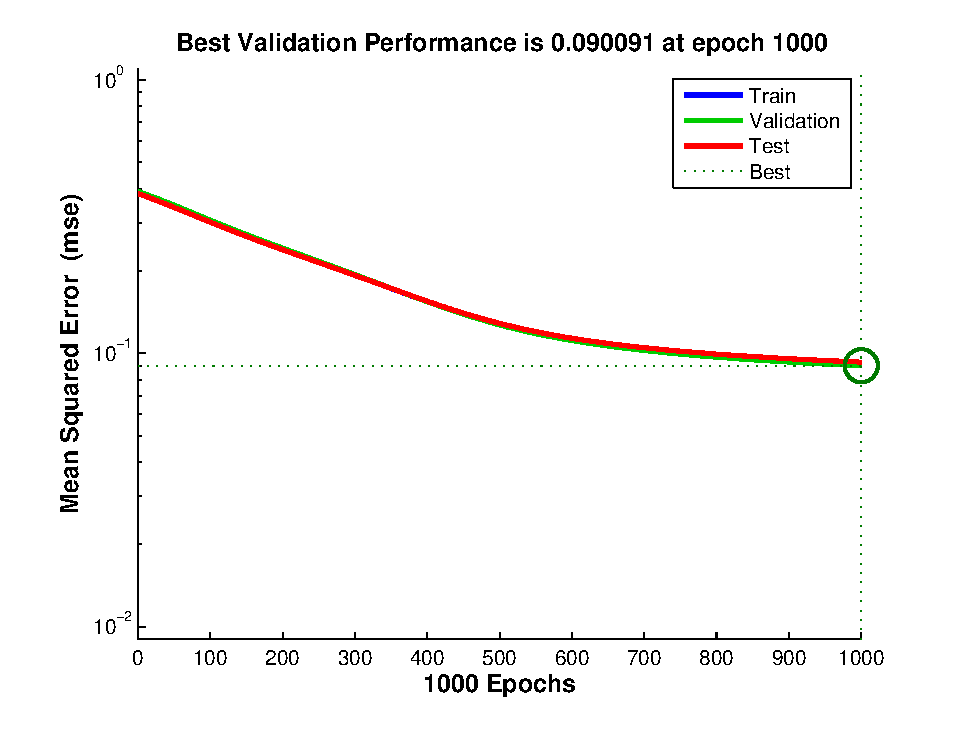
\includegraphics[scale=0.7]{eps/gradient-descent-performance.eps}
    \caption{Perfomance against epochs for \emph{Gradient Descent with Momentum} training function}
    \label{fig:gdm-performance}
    \end{figure}

    \subsection{Resilient Propagation}

    With this training function it is possible to have some enhancements respect the previous one, 
    as we can see from \autoref{fig:summary-table}, classification produces a samples' distribution
    where classes \emph{One} and \emph{Four} get increased, while the last two classes take no sample at all.

    Respect individual classes, taken a secret sample $s \in Two$ from the dataset, $s$ is correctly classified $82.83$ times out of $100$. 
    On the other hand, taken a secret sample $s \in Three$ from the dataset, $s$ is correctly classified $64.57$ times out of $100$;
    classification does a mistake for all other classes.

    In \autoref{fig:rprop-performance} we report a plot of performance against epochs: as we can
    see the error decreases faster than the previous training function's one, taking $147$ epochs to complete the learning.

    \begin{figure}
    \centering
    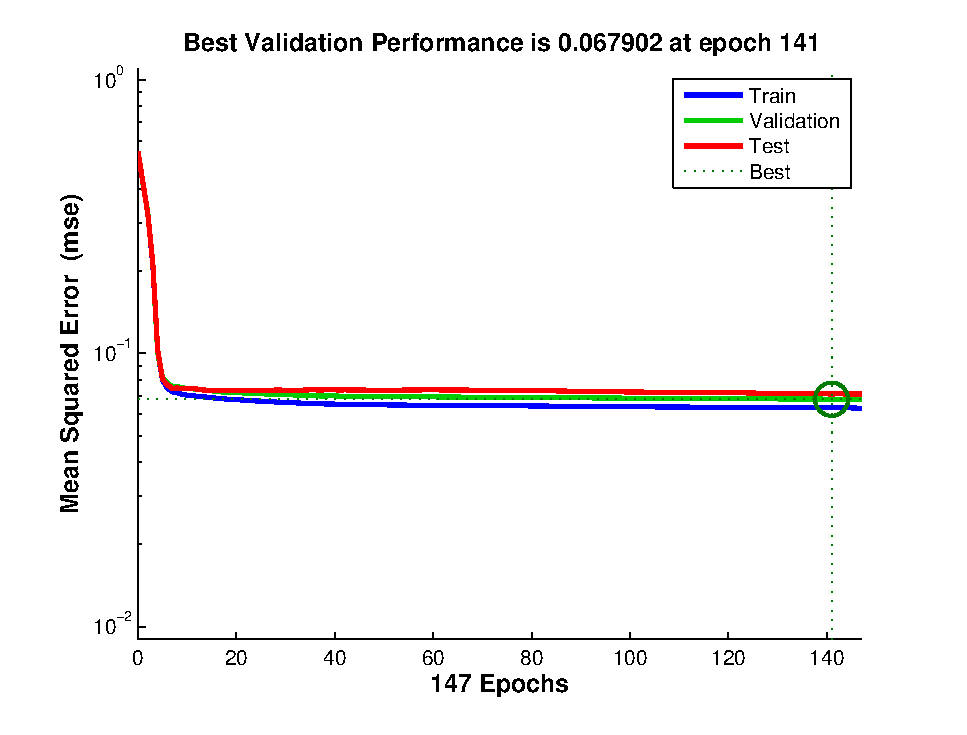
\includegraphics[scale=0.7]{eps/rprop-performance.eps}
    \caption{Perfomance against epochs for \emph{Resilient Propagation} training function}
    \label{fig:rprop-performance}
    \end{figure}

    \subsection{Scaled Conjugate Gradient}

    This training function produced quite surprising results, since it classifies secret
    samples in two classes only, \emph{Two} and \emph{Three} respectively. Maybe this strange behavior
    can be explained by the presence of some noise in the secret samples.

    In \autoref{fig:scg-performance} we report a plot of performance against epochs: as we can
    see the error decreases in two main steps, remaining ``constant'' in those steps,
     taking $30$ epochs to complete the learning.

    \begin{figure}
    \centering
    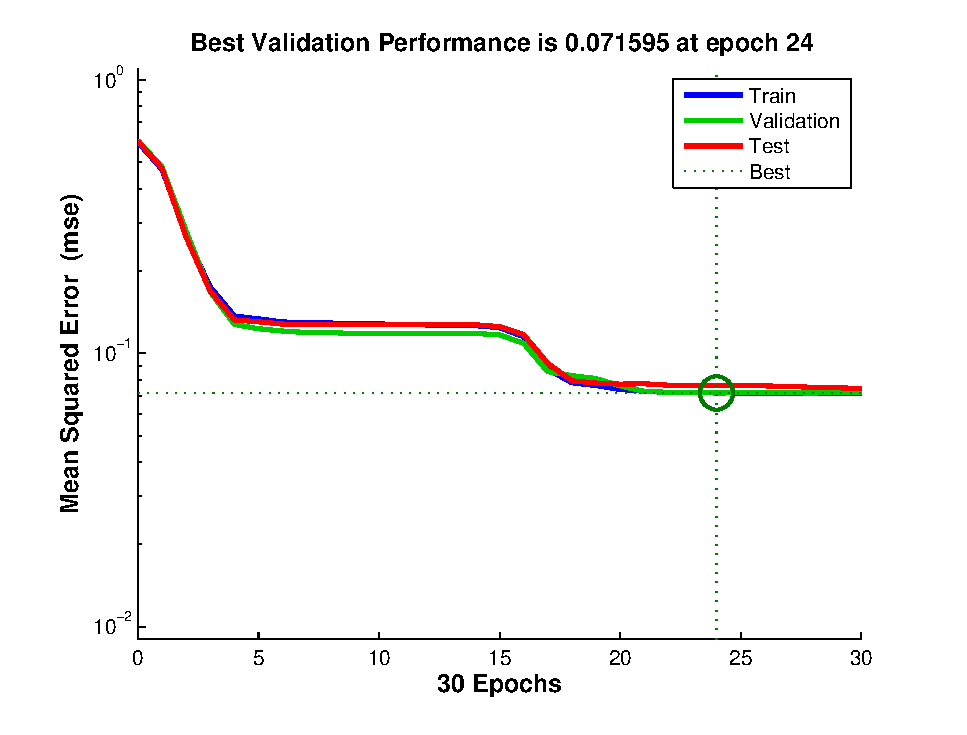
\includegraphics[scale=0.7]{eps/scg-performance.eps}
    \caption{Perfomance against epochs for \emph{Scaled Conjugate Gradient} training function}
    \label{fig:scg-performance}
    \end{figure}

    \subsection{Levenberg-Marquardt}

    This training function is the one that produces a samples' distributions quite similar 
    to the known ones, both for training samples both for samples kept secret. 

    Respect individual classes, taken a secret sample $s \in One$ from the dataset, 
    $s$ is correctly classified $54.29$ times out of $100$, while other trainings always behave worse. 
    Taken a secret sample $s \in Two$ from the dataset, $s$ is correctly classified $80.14$ times out of $100$. 
    On the other hand, taken a secret sample $s \in Three$ from the dataset, $s$ is correctly classified $69.18$ times out of $100$;
    classification does a mistake for all other classes.

    In \autoref{fig:lm-performance} we report a plot of performance against epochs: as we can
    see the error decreases very fast, taking $27$ epochs to complete the learning.

    \begin{figure}
    \centering
    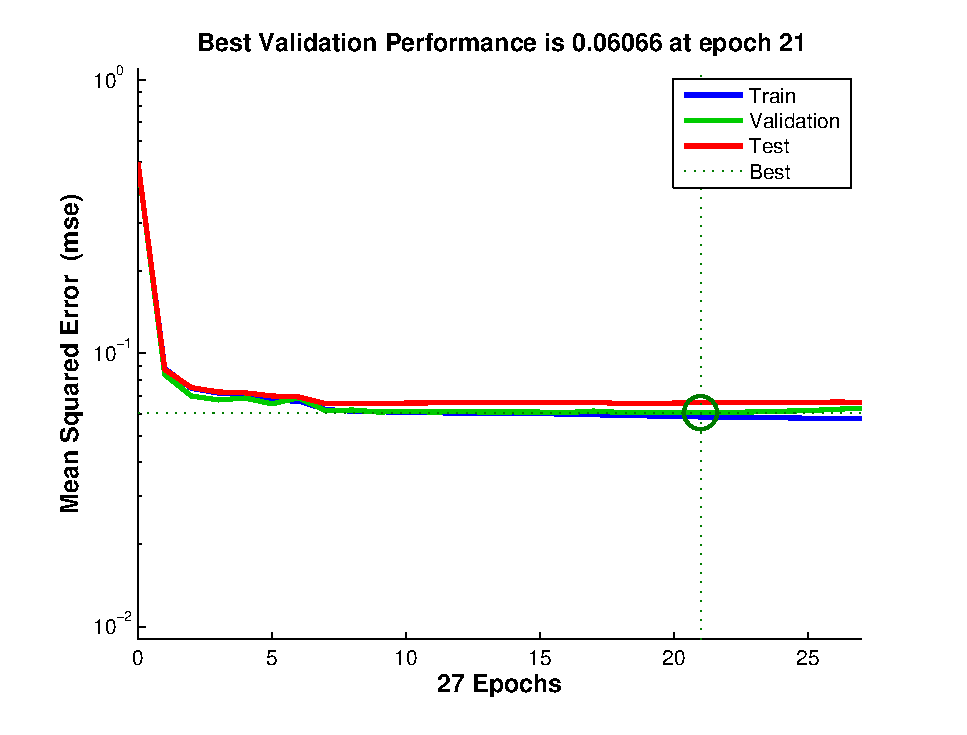
\includegraphics[scale=0.7]{eps/lm-performance.eps}
    \caption{Perfomance against epochs for \emph{Levenberg-Marquardt} training function}
    \label{fig:lm-performance}
    \end{figure}

    \section{Classification results}
    
    In general, the classifications we've experimented with doesn't behave very
    well, both respect the training samples both those kept secret: the 
    best training function is \emph{Levenberg-Marquardt} for our purpose.

    We could suggest that some improvements can be achieved if training consumes standardized
    data: we've tackled this approach writing a Matlab script 
    and then using the results as inputs for new experiments, obtaining better classification
    of secret samples. We do not report those results here since it's only a sketch work, 
    pointing the interested reader to  repository described in \autoref{sec:appendix}.


    \newpage

    \section{Appendix}
    \label{sec:appendix}

    \subsection{License}
\begin{verbatim}
The MIT License (MIT)

Copyright (c) 2014 Massimo Nocentini

Permission is hereby granted, free of charge, to any person obtaining a copy
of this software and associated documentation files (the "Software"), to deal
in the Software without restriction, including without limitation the rights
to use, copy, modify, merge, publish, distribute, sublicense, and/or sell
copies of the Software, and to permit persons to whom the Software is
furnished to do so, subject to the following conditions:

The above copyright notice and this permission notice shall be included in all
copies or substantial portions of the Software.

THE SOFTWARE IS PROVIDED "AS IS", WITHOUT WARRANTY OF ANY KIND, EXPRESS OR
IMPLIED, INCLUDING BUT NOT LIMITED TO THE WARRANTIES OF MERCHANTABILITY,
FITNESS FOR A PARTICULAR PURPOSE AND NONINFRINGEMENT. IN NO EVENT SHALL THE
AUTHORS OR COPYRIGHT HOLDERS BE LIABLE FOR ANY CLAIM, DAMAGES OR OTHER
LIABILITY, WHETHER IN AN ACTION OF CONTRACT, TORT OR OTHERWISE, ARISING FROM,
OUT OF OR IN CONNECTION WITH THE SOFTWARE OR THE USE OR OTHER DEALINGS IN THE
SOFTWARE.
\end{verbatim}

    \subsection{Project hosting}
    All the content of this project has been versioned in a \emph{Git} repository and 
    it is of public domain:\\
    \url{https://github.com/massimo-nocentini/neural-networks-exam}.\\

    All code developed in \emph{Pharo Smalltalk} is freely available at
    \url{http://smalltalkhub.com/#!/~MassimoNocentini/NeuralNetworksExam}
    and can be loaded directly via \emph{Monticello} smalltalk browser
    with the following message:
    \begin{adjustwidth}{-2cm}{}
    \begin{verbatim}
    MCHttpRepository
    location: 'http://smalltalkhub.com/mc/MassimoNocentini/NeuralNetworksExam/main'
    user: ''
    password: ''
    \end{verbatim}
    \end{adjustwidth}    
      
    \begin{thebibliography}{9}

    \bibitem{Nash-Sellers-Talbot-Cawthorn-Ford}
    Warwick J Nash, Tracy L Sellers, Simon R Talbot, Andrew J Cawthorn and
    Wes B Ford (1994) ``The Population Biology of Abalone (Haliotis
    species) in Tasmania. I. Blacklip Abalone (H. rubra) from the North
    Coast and Islands of Bass Strait'', Sea Fisheries Division, Technical
    Report No. 48 (ISSN 1034-3288)


    \bibitem{ml-berkeley-dataset-url}
      Abalone dataset,
      \url{http://archive.ics.uci.edu/ml/machine-learning-databases/abalone/abalone.data}.



    \end{thebibliography}

\end{document}
